\newif\ifshowsolutions
\showsolutionstrue
\documentclass{article}
\usepackage{listings}
\usepackage{amsmath}
%\usepackage{subfigure}
\usepackage{subfig}
\usepackage{amsthm}
\usepackage{amsmath}
\usepackage{amssymb}
\usepackage{graphicx}
\usepackage{mdwlist}
\usepackage[colorlinks=true]{hyperref}
\usepackage{geometry}
\usepackage{titlesec}
\geometry{margin=1in}
\geometry{headheight=2in}
\geometry{top=2in}
\usepackage{palatino}
\usepackage{mathrsfs}
\usepackage{fancyhdr}
\usepackage{paralist}
\usepackage{todonotes}
\setlength{\marginparwidth}{2.15cm}
\usepackage{tikz}
\usetikzlibrary{positioning,shapes,backgrounds}
\usepackage{float} % Place figures where you ACTUALLY want it
\usepackage{comment} % a hack to toggle sections
\usepackage{ifthen}
\usepackage{mdframed}
\usepackage{verbatim}
\usepackage[strings]{underscore}
\usepackage{listings}
\usepackage{bbm}
\rhead{}
\lhead{}

\renewcommand{\baselinestretch}{1.15}

% Shortcuts for commonly used operators
\newcommand{\E}{\mathbb{E}}
\newcommand{\Var}{\operatorname{Var}}
\newcommand{\Cov}{\operatorname{Cov}}
\newcommand{\Bias}{\operatorname{Bias}}
\DeclareMathOperator{\argmin}{arg\,min}
\DeclareMathOperator{\argmax}{arg\,max}

% do not number subsection and below
\setcounter{secnumdepth}{1}

% custom format subsection
\titleformat*{\subsection}{\large\bfseries}

% set up the \question shortcut
\newcounter{question}[section]
\newenvironment{question}[1][]
  {\refstepcounter{question}\par\addvspace{1em}\textbf{Question~\Alph{question}\!
    \ifthenelse{\equal{#1}{}}{}{ [#1 points]}: }}
    {\par\vspace{\baselineskip}}

\newcounter{subquestion}[question]
\newenvironment{subquestion}[1][]
  {\refstepcounter{subquestion}\par\medskip\textbf{\roman{subquestion}.\!
    \ifthenelse{\equal{#1}{}}{}{ [#1 points]:}} }
  {\par\addvspace{\baselineskip}}

\titlespacing\section{0pt}{12pt plus 2pt minus 2pt}{0pt plus 2pt minus 2pt}
\titlespacing\subsection{0pt}{12pt plus 4pt minus 2pt}{0pt plus 2pt minus 2pt}
\titlespacing\subsubsection{0pt}{12pt plus 4pt minus 2pt}{0pt plus 2pt minus 2pt}


\newenvironment{hint}[1][]
  {\begin{em}\textbf{Hint: }}{\end{em}}

\ifshowsolutions
  \newenvironment{solution}[1][]
    {\par\medskip \begin{mdframed}\textbf{Solution~\Alph{question}#1:} \begin{em}}
    {\end{em}\medskip\end{mdframed}\medskip}
  \newenvironment{subsolution}[1][]
    {\par\medskip \begin{mdframed}\textbf{Solution~\Alph{question}#1.\roman{subquestion}:} \begin{em}}
    {\end{em}\medskip\end{mdframed}\medskip}
\else
  \excludecomment{solution}
  \excludecomment{subsolution}
\fi

\newcommand{\boldline}[1]{\underline{\textbf{#1}}}

\chead{%
  {\vbox{%
      \vspace{2mm}
      \large
      Machine Learning \& Data Mining \hfill
      Caltech CS/CNS/EE 155 \hfill \\[1pt]
      Miniproject 1\hfill
      Released January $28^{th}$, 2017 \\
    }
  }
}

\begin{document}
\pagestyle{fancy}

% LaTeX is simple if you have a good template to work with! To use this document, simply fill in your text where we have indicated. To write mathematical notation in a fancy style, just write the notation inside enclosing $dollar signs$.

% For example:
% $y = x^2 + 2x + 1$

% For help with LaTeX, please feel free to see a TA!



\section{Introduction}
\medskip
\begin{itemize}

    \item \boldline{Group members:} Enrico Borba, Claire Goeckner-Wald \\
    % Insert text here.

    \item \boldline{Team name:} Papa Mart's Mini Gary (for 2008), Papa Mart's
    Giant Gary (for 2012). \\
    % Insert text here.

    \item \boldline{Division of labour:} \textbf{Enrico Borba:} programming, tweaking numbers; \textbf{Claire Goeckner-Wald:} model suggestion $\&$ research of models,
    compilation of report.\\
    % Insert text here.

\end{itemize}



\section{Overview}
\medskip
\begin{itemize}

    \item \boldline{Models and techniques tried}
    \begin{itemize}
    % Insert text here. Bullet points can be made using '\item'. Models and techniques should be bolded using '\textbf{}'.
    \item \textbf{Neural networks:} Attempted one-hot encoding across all
        features, attempted different optimizers. Determined ineffective at
        categorical data.
    \item \textbf{Decision trees:} Attempted different kinds of trees. Extremely
        random trees, random trees.
    \item \textbf{Ensembles:}
        Mostly focused on ensembles of extremely random trees. The most effective
        of which was 500 trees with a min_samples_split of 11.
        \\
        Ensembles of different models were also attempted, specifically,
        Linear SVM + Neural network + Extremely random tree with little
        success.
    \item \textbf{SVMs:}
        Tried two different kernels, rbf and linear. RBF kernel was deemed
        unusable from the beginning due to its more than quadratic runtime
        complexity for training (with respect to the number of data points).
    \item \textbf{Cross-validation:}
        Main method for determining the strength of a model.
    \item \textbf{Removing unecessary columns:}
        Columns that had more than 95\% BLANK responses (-1), were removed
        entirely from the input data before training and before predicting.
    \item \textbf{Data normalization:}
        Normalizing data before training and prediction.
    \end{itemize}

    \item \boldline{Work timeline}
    \begin{itemize}
    % Insert text here. Bullet points can be made using '\item'.
    \item \textbf{Week 1:} Discussing models, setting up data inputs
    \item \textbf{Week 2:} Github repo, Cross-validation of models to determine which was best, determining which data columns were unnecessary, researching other models, and final submissions
    \end{itemize}

\end{itemize}

\pagebreak

\section{Approach}
\medskip
\begin{itemize}

    \item \boldline{Data processing and manipulation}
    \begin{itemize}
    % Insert text here. Bullet points can be made using '\item'.
    \item \textbf{Feature Pruning:} When inspecting the input data, we quickly
    see that there are several BLANK (-1) entries. So, we were willing to
    try to prune some features, depending on the proportion of BLANK responses
    in that specific feature. \\

    Here is a graph representing this behavior, and the extent of pruning.

    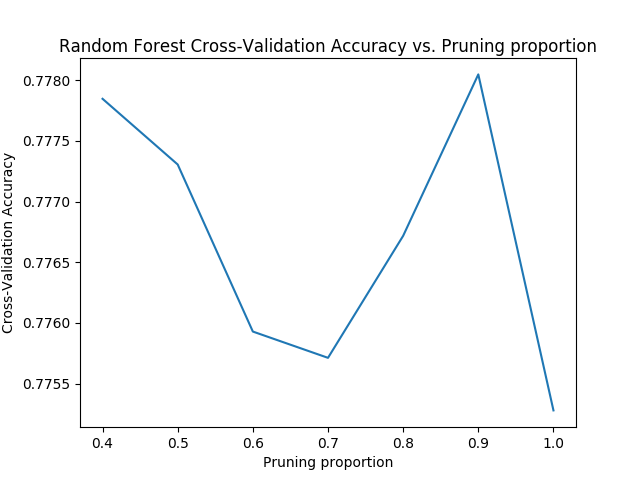
\includegraphics[width=30em]{figure_1.png}

    The model being trained is a random forest with min_samples_split=4 (a
    detailed explanation given on page 4). The x-axis is the
    tolerance of pruning. That is, if x = 0.9, then features for which the
    proportion of BLANK responses is greater than 0.9 are pruned. The y-axis
    is the mean validation accuracy in 3-fold cross validation. The data is
    not shuffled, so the same sets of inputs are used for each model being
    trained.\\


    \item \textbf{Data Normalization:}
    We determined normalization was not extremely useful in increasing
    classification accuracy when using decision trees.
    For an Extremely random forest of 100 trees, we
    had cross validation accuracy with normalization: 0.757032214087
    and without: 0.772078501506.

    \end{itemize}

    \pagebreak

    \item \boldline{Details of models and techniques}
        \begin{itemize}
    % Insert text here. Bullet points can be made using '\item'. Models and techniques should be bolded using '\textbf{}'.
    \item \textbf{Neural networks:}
        Neural networks did not immediately seem useful, as we felt that we
        would have to one-hot encode every feature, and we believed it would
        be surpassed by decision trees in classification. \\

        We wanted to test the strength of a neural network. We generated 100
        random neural networks of the form:
        \begin{center}
            \begin{tabular}{ c c c }
                \hline
                Layer (type) & Output Shape & Number of Parameters \\
                \hline
                Dense & $d_1$ & $p_1$ \\
                Activation & $d_1$ & 0 \\
                Dropout & $d_1$ & 0 \\
                \hline
                Dense & $d_2$ &  $p_2$ \\
                \vdots & \vdots & \vdots \\
                \hline
                Dense & 3 & $p_n$ \\
            \end{tabular}
        \end{center}
        The number of hidden layers ranged from 10 to 20 and the number of
        neurons in each layer ranged from 300 to 600. We normalized and
        one-hot-encoded all features and outputs. The activation layers were
        randomly selected to all be either tanh, sigmoid, or ReLU. Furthermore,
        the dropout was one of 0.1, 0.2, \dots, 0.5. \\

        The strongest neural network had a cross-validation error of 0.737165. \\

        We quickly noticed that the neural network was merely learning to
        always output ones. The 2008 training dataset contained 0.745\% ones,
        in the PES1 column. Thus, the best neural network was doing worse than
        simply outputting ones.

    \pagebreak

    \item \textbf{Decision Trees/Ensembles:}
        We had two tree classifiers in mind: RandomForestClassifier and
        ExtraTreesClassifier. Both were provided by sklearn.Both of these
        classifiers are ensembles of decision trees. \\

        ExtraTreesClassifier fits
        a number of randomized decision trees (a.k.a. extra-trees) on various
        sub-samples of the dataset and use averaging to improve the predictive
        accuracy and control over-fitting. \\

        RandomForestClassifier fits a number of decision tree classifiers on
        various sub-samples of the dataset and use averaging to improve the
        predictive accuracy and control over-fitting. \\
        \begin{itemize}
            \item \textbf{ExtraTreesClassifier:}
                We first wanted to test the proper regularization parameter
                for ExtraTreesClassifier. We tested different values for
                the minimum number of samples required to split an internal
                node. We had min_samples_split range from 2 to 14, and the
                y-axis is the cross-validation error of 3 folds. \\

                We also wanted to test the min_samples_leaf, the minimum number of
                samples required to be at a leaf node. Again, the Training
                accuracy is a cross-validation error of 3 folds.
                \begin{center}
                    \begin{tabular}{ c c }
                    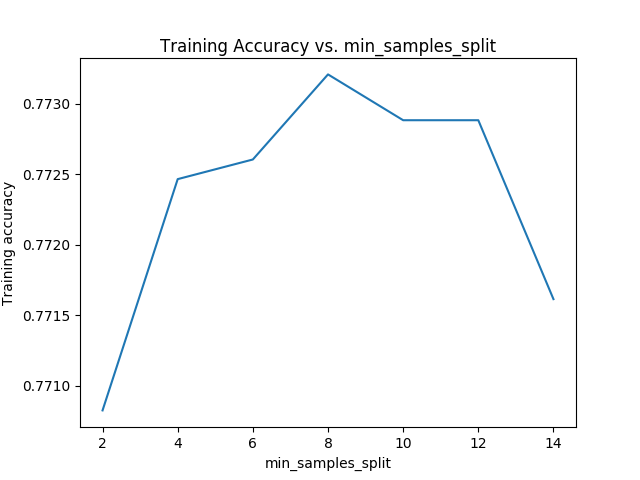
\includegraphics[width=20em]{figure_3.png} &
                    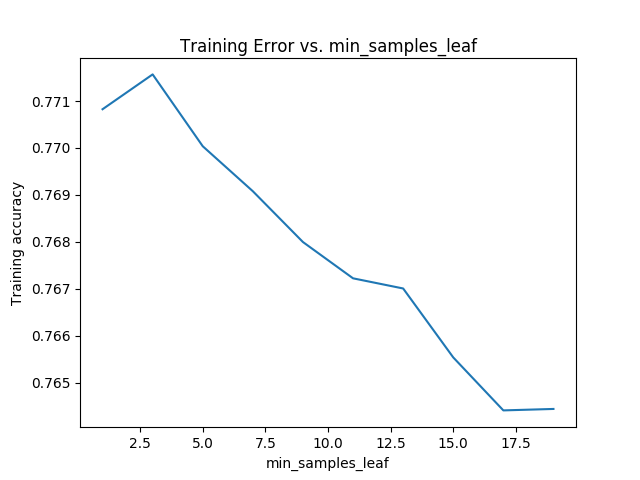
\includegraphics[width=20em]{figure_4.png}
                    \end{tabular}
                \end{center}
                We see the strength of the model is maximized when
                min_samples_split is 8, and when min_samples leaf is 3.\\

                The combination of the two with an 100 tree ensemble yields a
                cross-validation accuracy of approximately 0.77342, a clear
                improvement over the neural network. With 500 trees, the
                cross-validation accuracy increases to 0.77389. A small but
                still clear improvement.

            \pagebreak

            \item \textbf{RandomForestClassifier:}
                We attempted the same experiment with the
                RandomForestClassifier, with interesting results.
                \begin{center}
                    \begin{tabular}{ c c }
                    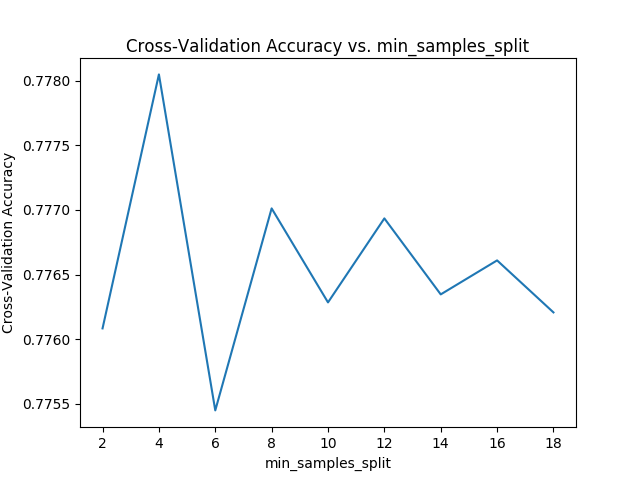
\includegraphics[width=20em]{figure_6.png} &
                    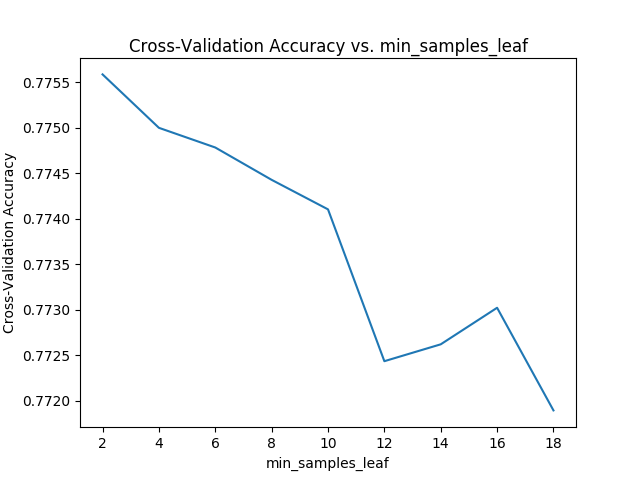
\includegraphics[width=20em]{figure_7.png}
                    \end{tabular}
                \end{center}
                It seems that regularization should be very small when
                using the RandomForestClassifier. \\

                Using min_samples_split = 4 and min_samples_leaf = 2, with
                500 trees we achieve a cross validation accuracy of
                0.77704, noticeably higher than that of the extremely random
                tree.

        \end{itemize}

    \item \textbf{K-Nearest Neighbors:}
        We also shortly investigated KNeighborsClassifier from sklearn, to see
        if the data had similar points in clusters. This ended up being
        very much not the case, as we can see in this graph here.
        \begin{center}
            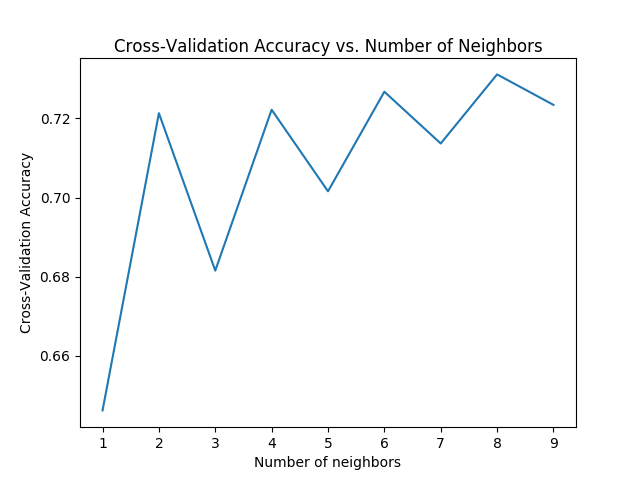
\includegraphics[width=30em]{figure_5.png}
        \end{center}
        We see that the strongest $k$-nearest neighbor classifier had a
        validation accuracy of 0.74449, far from that of the extremely
        random tree ensemble.

    \pagebreak

    \item \textbf{SVMs:}
        \begin{itemize}
            \item \textbf{RBF Kernel:}
            We were interested in training the rbf kernel support vector machine,
            specifically sklearn's svm.SVC(). However, the computational complexity
            of training is greater than

            $$O(n_\text{features} \times n_\text{observations}^4)$$\\

            Therefore, we could not train on more than 10000 points. Because of
            this, we were already sure that we would not use the rbf kernel
            svm, since it could not train on the entire dataset, however, we
            still wished to determine its strength. \\

            Training on
            a random 10000 points in the dataset and using the rest as a validation
            set yielded 0.75350 as the test error. Unfortunately, not much better
            than the neural network, and definitely worse than the extra random
            tree classifier.\\

            \item \textbf{Linear Kernel:}
            We also tried a linear kernel. Since it's training computational
            complexity is linear in the number of observations, it could be
            evaluated on the entire dataset. The linear kernel has a
            cross-validation error of 0.52452, implying the data is far from
            linearly seperable.
            Fitting the linear kernel was worse than guessing one always. This
            seems very counter intuitive, as the hyperplane with the least
            error should be one that is simply entirely outside of the whole
            dataset.
        \end{itemize}
    \end{itemize}

\end{itemize}



\section{Model Selection}
\medskip
\begin{itemize}

    \item \boldline{Scoring} \\
    We selected from the models described above. The metrics the models were
    scored on varied from metric to metric (specifically, the loss functions
    differed in each model). For Neural Networks, the Nesterov Adam (Adam
    optimizer with momentum), was the optimizer that fared best. We used
    categorical_crossentropy as the loss parameter when training the
    neural networks.\\

    For the decision trees, (both the extra random and the
    regular random forests) used Gini index as a metric for impurity. \\

    The $k$-nearest neighbors classifier used sklearn's BallTree algorithm
    for training.\\

    For the support vector classifiers we attempted both a linear and the
    radial-basis function kernels, with little success. \\

    It was clear that the Random Forest was the most promising classifier.

\pagebreak

    \item \boldline{Validation and Test} \\
    Cross validation (3 fold) was used to determine the strength and selection
    of all models. For the Extremely Random Tree and Random Forest Classifiers,
    we refined the measurement and used 10 fold validation. We came to the
    same result that the RandomForest was slightly stronger.

\end{itemize}



\section{Conclusion}
\medskip
\begin{itemize}

    \item \boldline{Discoveries} \\
    We discovered the intuitive fact that some columns contain worthless
    information, and will only hinder learning. Removing these columns
    carefully has a visible positive effect on the strength of the model. \\

    Neural networks are not extremely powerful classification problems which
    have discrete inputs, unless each feature is one-hot encoded.
    Decision trees are much more effective at these kinds of problems.

    \item \boldline{Challenges} \\
    We had a lot of challenge improving the model moderately after achieving a
    classification of about $0.778\%$. We also had difficuly in implementing
    boosting.

    \item \boldline{Concluding Remarks} \\
    If given more time, boosting would have been properly implemented with
    a random forest as the model being boosted. This would have also had a
    strong positive impact in the strength of the final model.\\

    The final model chosen was a Random Forest with min_samples_split=4 of
    1000 trees.


\end{itemize}



\end{document}